
\chapter{Estimation: Advanced Glance on the Question}
\section{Weighted MLE}
\subsection{Theory of Weighting}
In the previous section, we got the formula of the MLE for a multidimensional ($ M \in \mathbb N^*$) Hawkes process, defined on the interval $[0,T]$, with jumps at times: $ \forall m \leq M: 0 < t_{1}^m \cdots < t_{n_m}^m \leq T $.

We recall that $ \Tau^m $ is referring to the list history, including the jumps' time $( t_{1}^m, \cdots , t_{n_m}^m ) $, and the marks; $\Theta$ represents the set of parameters of the process. Finally, the superscript visible on $L^m$ is mentioned in order to avoid confusion between each likelihood function of each marginal process (with respect to the multi-dimensional Hawkes process). 

The marginal log-likelihood reads (cf. eq. (\ref{eq:intensity_lambda})):


\begin{equation}
\ln L^m( \Theta \mid \Tau ) = - \int_0^T \lambda^{m} ( s \mid \Theta , \Tau ) ds + \int_0^T \ln \lambda^{m}( s \mid \Theta , \Tau ) d N_s^m \label{eq:log_likelihood}
\end{equation}



In section II from \cite{weighted_likelihood}, and by coining the weight function $w$\footnote{also called in the following kernel. We will introduce a difference of realm between the two in the next section in footnote \ref{section:diff_kernel_weights}. Since the difference is quite subtle, we use weights, kernel and window interchangeably.}, they define the weighted estimating equation as:

\begin{equation}
\ln W L ( \Theta \mid \{ X_1, \cdots, X_n \} ) = \sum_1^n  w(X_i) \ln f( X_i \mid \Theta ) 
\end{equation}

We emphasize on the notation WL to highlight the spirit of the weighted likelihood estimation problem, which is different from the classic likelihood estimation problem.


In our case scenario, we add up a time dependence upon the kernel, and replace the $\sequence{X_i}$s by $\sequence{t_i}$s.


Remember that we had from eq. (\ref{eq:ln_multi}):
 
\begin{equation}
\ln L( \Theta \mid \Tau ) = \sum_1^M \ln L^m( \Theta \mid \Tau )
\end{equation}

And this is also true for the weighted likelihood. Hence, focusing on our marginal weighted likelihood, the estimating equation reduces to:



\begin{align}
\ln W L^m( \Theta \mid \Tau ) &= - \int_0^T w(s) \lambda^{m} ( s \mid \Theta , \Tau ) ds + \int_0^T w(s) \ln \lambda^{m} ( s \mid \Theta , \Tau ) d N_s^m  
\label{eq:weighted_log_likelihood} \\
&=  - \int_0^T w(s) \lambda^{m} ( s \mid \Theta , \Tau )  ds +  \sum^{n_m}_i  w(t_i) \ln \lambda^{m} ( t_i \mid \Theta , \Tau )  \label{eq:weighted_log_likelihood2} 
\end{align}

Notice how if all the weights are equal to unity, the resulting estimator is the usual maximum likelihood estimator, i.e. if $w \equiv 1$, then eq. (\ref{eq:weighted_log_likelihood}) becomes eq. (\ref{eq:log_likelihood}). We wrote down explicitly eq. (\ref{eq:weighted_log_likelihood2}) in order to emphasize how the kernel function becomes random through the jumps' time $t_i$. 

Weighting should be a way to rescale the information at our disposal. For that reason, we restrict the set of considered kernels to be of norm $T$:

$$\Omega_w := \{ w \colon \mathbb R \to \mathbb R, \text{ such that : } \norm{w}_{L^1 } = T \} $$

Notice that for the non-weighted case, when $w \equiv 1$, its norm is equal to $T$. By this, we ensure that we conserve, using the physical expression, the energy of each integrand. That's the reason why we fix the value of the norm of every kernel inside $\Omega_w$ to $T$. Also, we do not need any other restriction on the considered functions. However, one usually considers fixing as well the positivity of kernel and its first moments, for identifiability reasons\footnote{These conditions ensure that the kernels are densities, an enjoyable feature when one estimates densities.}. 

\subsection{Advantage and Notation of WMLE}

The idea behind using weighted likelihood is that by using a non-constant weight function, solving for the maximum likelihood estimator given by eq. (\ref{eq:weighted_log_likelihood}) can potentially outperform the one given by eq. (\ref{eq:log_likelihood}). 

Essentially, we want to take advantage of the fact that a larger weight w(s) gives to observations in the infinitesimal region $ds$ more influence on the estimation process. This would allow us to estimate parameters that are time dependent by adding that dependence within kernels. Now the main question shall be which kernel should we chose. Recall what Silverman said in \cite{Silverman} at page 43:

\vspace{0.5cm}
\textit{It should never be forgotten that the appropriate choice of smoothing parameter will always be influenced by the purpose for which the density estimate is to be used. }
\vspace{0.5cm}

One should be careful about the choice of the kernel. Let's think about the two extreme cases for weights: 

\begin{enumerate}
\item A constant kernel considers all the jumps equally and hence, computes an estimator that estimates the average over the whole simulation time $[0,T]$. Overall, the bias will be high, but the variability low.
\item A kernel that considers only a small region will give a very precise estimate for that given region, but with much more variability over the time.
\end{enumerate}

This phenomenon is due to the well-known bias/variance trade-off.
\label{section:bias-variance_trade-off}

\label{section:kernel_weights_first_conversation}
In the rest of the chapter, we delve into the choice of such windows in order to optimize the performances of the WMLE. Our aim being to estimate parameters that are time dependent. We add that dependency to the WMLE through the kernel, which should be written consequently $w_t$. However, for clarity, it will be kept as $w$. We need to mention an important matter in order to avoid any confusion. Our weight function is evaluated at the points $\sequence{t_i}$ when the jumps of the Hawkes process occur. Also, the time dependence is introduced by centring the kernel around $t$ by a classic substitution: 

$$w(t_i) \to w(  t_i - t ) $$

For the same reasons of clarity, we are not going to write this change of variable inside $w$. Also, the times $t$ at which we want to estimate the parameters can't be coined as $\sequence{t_i}$ since it is already our notation for the jumps' time. Hence, we will write these times as $\sequencetime$.

In the following, we are going to delve into the theory of KDE, where it is common to use the letter $K$ instead of $w$. Also, the objective in KDE is slightly different. KDE's aim is to find the estimate of a function $f$ evaluated at the point $t$ by using kernels centred around $t_i$. For that reason, people are using kernels with the following substitution:

$$ K(t) \to K(t - t_i)$$

Hence, in order to avoid confusion, we keep for a few theoretical sections the notation $K$ for kernels, for which we write the substitution. 

Later, we do propose a definition in section \ref{section:equivalence_bi_rep} that splits the two objects into distinct concepts.


\subsection{WMLE Algorithm}
In order to go from the MLE to the WMLE, we need to add the weights inside the computations. The necessary adaptation one has to do is to multiply the contribution of each jump to the log-likelihood by the corresponding weight. As long as the weights are $\alpha, \beta, \nu$-independent\footnote{Ensuring that the derivatives do not change, up to a multiplicative constant.}, it is the only difference we have to include.  

The idea of mixing the dependency of the parameters inside the weights in order to improve performances is something that could be done. It would basically be parametrizing the MLE. If for instance we are estimating the parameter at $t_2$ with $t_1 < t_2$, an idea could be to use the already done estimation at $t_1$ for computing the estimation at $t_2$.



\section{Choice of the Window}

We mentioned our wish of estimating the parameters with some time-dependence. By inspiring ourselves from kernel density estimation (KDE) theory, we hope to be also able to estimate correctly the evolution of the parameters through time. The main difference between KDE and our task is that our estimate won't be a density function\footnote{Hence, the integral of the function does not have to yield $1$. However, notice that the condition set on our model ensures that all parameters are positive, thus, the functions are always positive}. 

In the following, we consider solely $1$-D kernels, which are weighting the maximum likelihood estimation\footnote{Kernels are by definition density functions usually coined in the literature by the symbol $K$. On the other hand, we are interested in weights $w$. For the following theoretical bit, we keep the notation from KDE since it is where the ideas come from. However, without loss of generality, one can scale kernels in order to get weights back. Thus, kernels are to weights what probability measures are to measures\label{section:diff_kernel_weights}.}. The latter leads to a parameter $\theta^* \in \Theta$, the MLE, which belongs to $\mathbb R^{m+2 m^2}$. We shall also underline on the variable the dependency on time $t$ with a subscript, which comes from the evaluation of the kernel at a precise time. If the variable $t$ was continuous, we would hence have a function $$\theta^*_t \colon \mathbb R  \to R^{m+2 m^2} $$

We would like to find the such best function, with respect to certain criteria, with respect to the choice of the kernel. For the theoretical part, we will look at a real-valued function $f$ without loss of generality. Indeed, defining an operator on $f$ is equivalent to define an operator on $\norm{\theta^*_t}$ where $\norm{\cdot}$ is any norm equipping $\mathbb R$.
\label{section:multi_to_uni}
\label{section:kernel_to_weights}






\subsection{Measure of Accuracy}
The class $ \Omega_w $ of functions is pretty big, and we would like to find the best kernels. For that reason, we first need to fix a metric in order to compare the scores of the different estimations. If one knows the true function estimated $f$, and calls the estimation $\hat{f}$, then one measure of accuracy is given by the mean square error, computed by: 

\begin{equation}
\MSE ( \hat{f}(u) ) \triangleq  \E [ ( \hat{f}(u) - f(u) )^2 ]
\end{equation}

whose global natural extension is given by the $L^1$ norm of the previous quantity, yielding the so-called mean integrated square error:

\begin{equation}
\MISE ( \hat{f}(u) ) \triangleq  \E [ \int ( \hat{f}(u) - f(u) )^2 du ]
\end{equation}

\begin{remarque}
One can rewrite, under mild condition of regularity:
\begin{align*}
\E [ \int ( \hat{f}(u) - f(u) )^2 du ] &= \int \E [( \hat{f}(u) - f(u) )^2 ] du \\
&= \int  \E[ (\hat{f}(u) ] - f(u) )^2 ] du + \int \Var( \hat{f}(u)) du 
\end{align*}
hence we came back to the classic bias-variance trade-off we already mentioned in section \ref{section:bias-variance_trade-off}.
\end{remarque}

Using the theory available in KDE, we are going to find the best kernels with respect to $\MISE$.

\section{Fixed Width Window}
\label{section:FWW}
\subsection{Optimal Kernel}

As exposed in \cite{Wand}, it is possible to derive the optimal kernel for KDE. In \cite{Wand}, the formula for asymptotical mean square error is given by their eq. (2.12). The issue here is that the scaling of $K$ is coupled with the bandwidth $h$. However, by a substitution inside $K$ of the form 
$$ K_{\delta} ( \cdot ) = \frac 1  {\delta } K \left ( \frac {\cdot } { \delta } \right ) $$
we get a factorization of the previous expression with separate dependency of the bandwidth and of the kernel. One has to simply choose $\delta$\footnote{Independent to $h$.} to be: $$ \delta_0 = \left ( \frac{ \int K(t)^2 dt }{ \left ( \int t^2 K(t) dt \right )^2 } \right ) ^{\frac 1 5} $$


\begin{theoreme}{Optimal kernel for KDE estimation choice}

\begin{equation}
\begin{array}{lcr}
\min_{ K  }  & C(K) := ( \mu_2 ^2 \cdot \norm{K}_{L^1}^4 )^{1/5}      &     \\
\text{subject to }   & K \geq 0 & \text{(positivity) } \\
& \norm{K}_{L^1} \triangleq  \int K = 1  & \text{(normalized)} \\
 & \mu_1 \triangleq  \int t K(t) dt = 0    & \text{(centred)                 } \\
& \mu_2 \triangleq  \int t^2 K(t) dt =: a         & \text{(finite second moment)   }           
\end{array}
\end{equation}

has the following class of kernels as a solution:

\begin{equation}
K^*_a(t) := \frac 3 4  \frac { 1 - \frac {t^2}{5 a^2} } {\sqrt{5} a } \11charac_{ \{ \abs t \leq \sqrt{5} a \} }
\end{equation} 

We usually refer to this class of kernel as Epanechnikov. It also is usual to fix $a=1$ and to rescale the kernel such that it is defined on $\abs t \leq 1 $, yielding:


\begin{equation}
K^*(t) := \frac 3 4 ( 1 - t^2 )  \11charac_{ \abs t \leq 1 }
\end{equation} 
\end{theoreme} 

The kernel that minimizes the target equation in the minimization problem is also the one which minimizes the $\MISE$. Actually, the quantity $C(K)$ is the kernel dependent part of the expression. 

Another popular scaled kernel, with almost equal performances is the biweight kernel defined as:

\begin{equation}
K_b(t) := \frac {15}{16} ( 1 - t^2 )^2  \11charac_{ \abs t \leq 1 }
\end{equation} 

\begin{remarque}
Note that the biweight kernel is of class $\mathcal C^{1}$ at $\{-1, 1\}$ while Epanechnikov isn't derivable at those points.
\end{remarque}











In order to compare the performances of different kernels, statisticians developed the concept of efficiency:

\begin{definition}[Efficiency of $K$ relative to $K^*$]
Efficiency represents the ratio of sample sizes necessary
to obtain the same accuracy when using $K^*$ as when using $K$. The efficiency is, thus, computed as:

$$ \left ( \frac{C(K^*)}{C(K)} \right ) ^{\frac 5 4 } $$
\end{definition}

Is shown page 31 in Table (2.1), in \cite{Wand}, Epanechnikov kernel has an efficiency of $1$, and the biweight has an efficiency of $0.994$. It is actually surprising how the windows aren't affecting efficiency in a very impactful manner.



\begin{remarque}
Four of the common kernels are actually derived with the same formula. They are all part of the same family:

$$ K(x,p) = \frac{(1-x^2)^p}{2^{2p+1} B(p+1,p+1) } \11charac_{\abs x < 1 }$$

where $B(\cdot, \cdot)$ is the beta function. Notice that $p=1$ corresponds to the Epanechnikov kernel, $p=2$ corresponds to the biweight kernel, $p=3$ matches with the often called triweight kernel and finally the limiting case of $p \to \infty$ corresponds to the standard normal density kernel. 
\end{remarque}


\begin{figure}
\centering
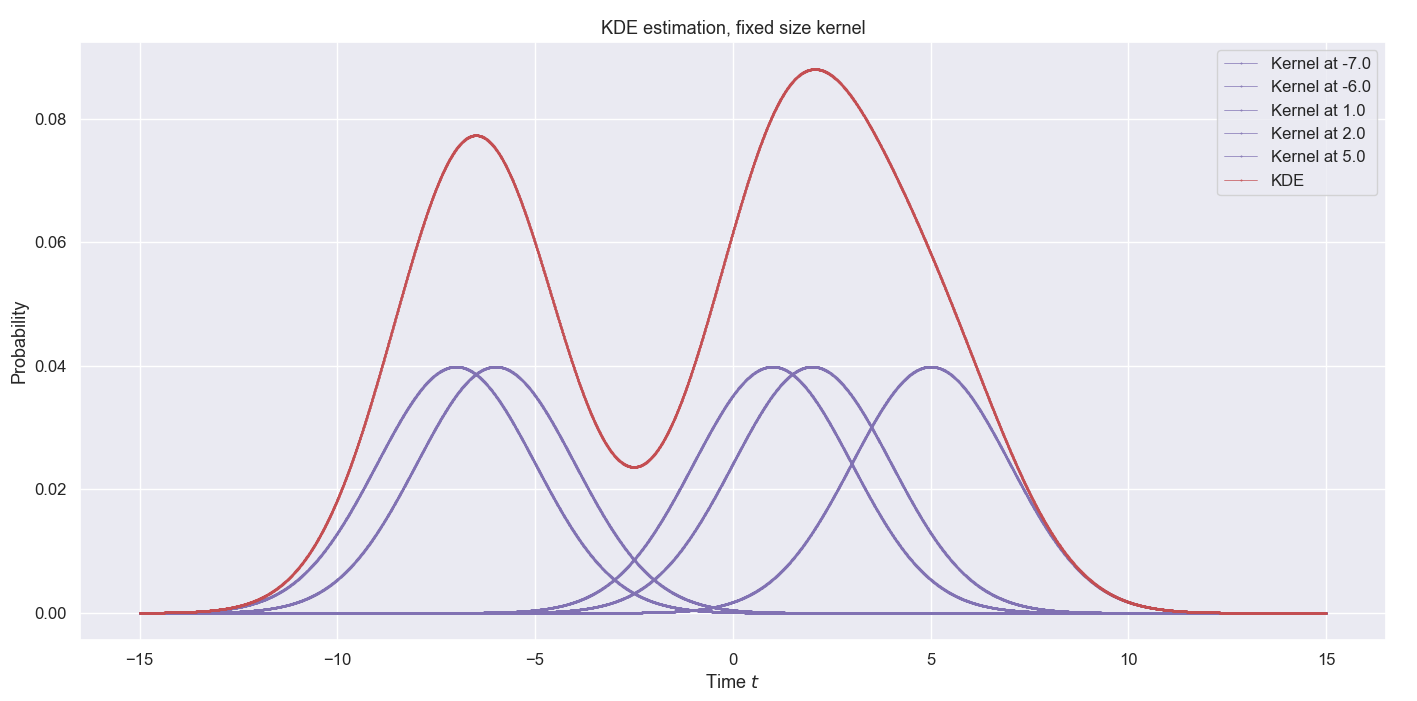
\includegraphics[width = 0.90 \textwidth]{../imag/chap3/FKDE.png}
\caption{Example of a fixed kernel density estimation, showing the impact of the single kernels.}
\label{fig:FKDE}
\end{figure}

\subsection{A Few Kernels That We Tried to Use}
\label{section_few_trials_kernels}

We tested the different discovered kernels for WMLE. We would like to see the impact of kernel's choice upon it. Since we haven't discussed the optimal width yet, we fix it to some arbitrary medium value. We discuss that question in the next subsection.

By considering parameters that are constant through time, as displayed on fig. \ref{fig:evol_choice_basic}, we tested different kernels, for fixed width, essentially the one from fig. \ref{fig:kernels_list}. We got the results from fig. \ref{fig:basic_5_kernels_alpha}, \ref{fig:basic_5_kernels_beta}, \ref{fig:basic_5_kernels_nu}. We did not notice any remarkable change. Perhaps it would be interesting to compute the change in MSE depending on the kernel. For now, this confirms our idea that the kernel's choice doesn't impact the estimation too much.


\begin{figure}
\centering
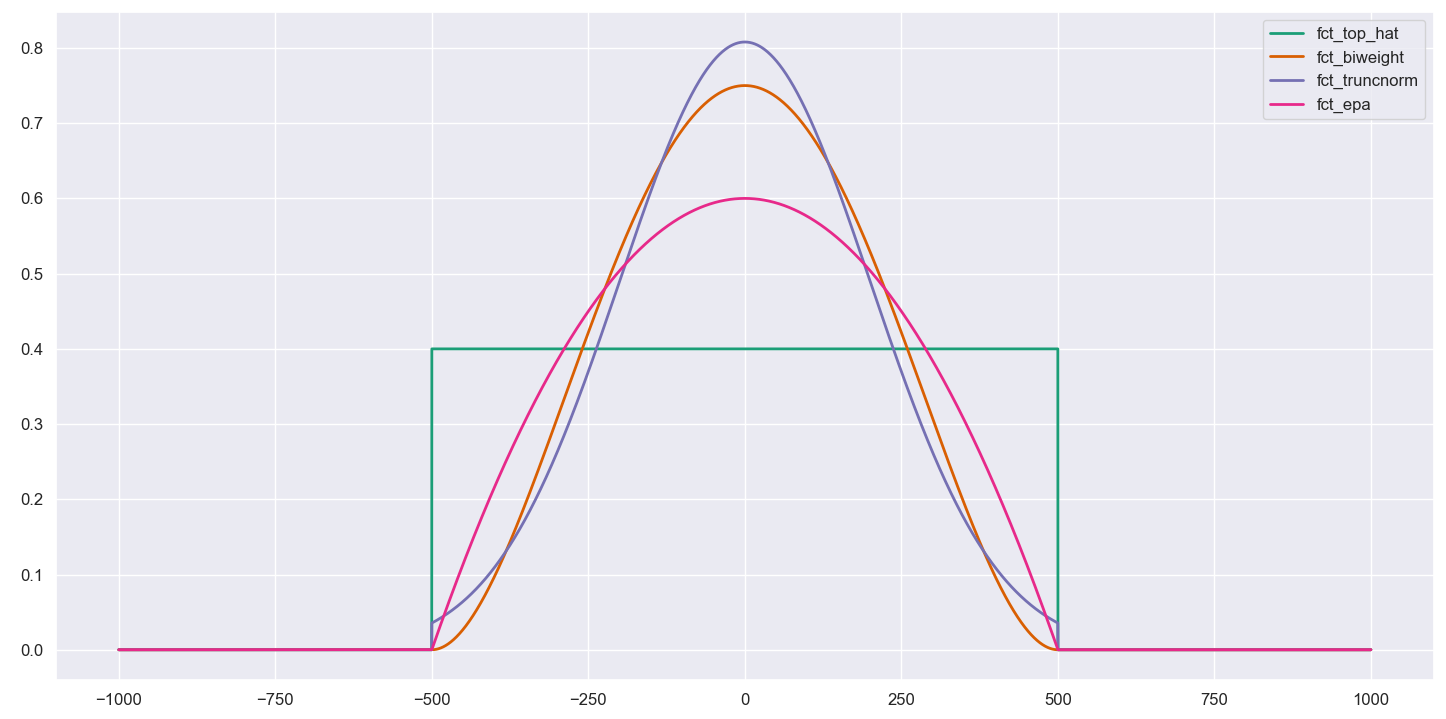
\includegraphics[width = 0.80 \textwidth]{../imag/chap3/the_kernels.png}
\caption{Superposition of the kernels shapes we mentioned.}
\label{fig:kernels_list}
\end{figure}


\begin{figure}
\centering
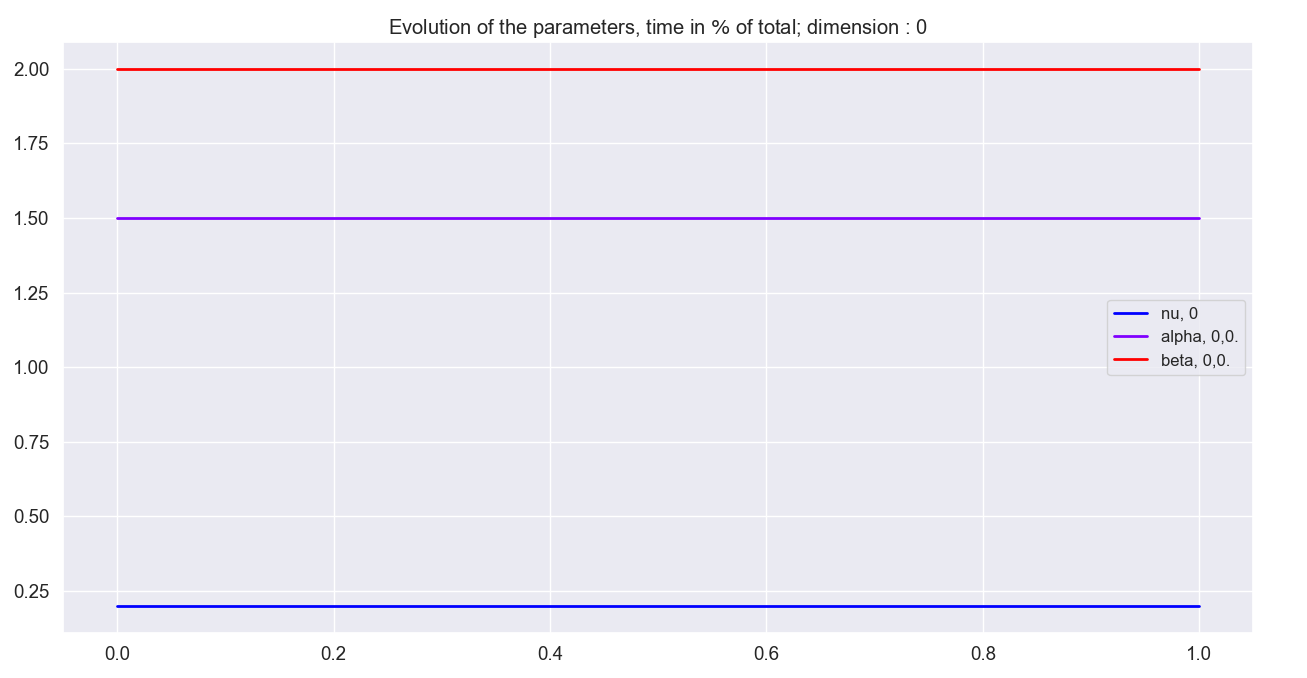
\includegraphics[width = 0.75 \textwidth]{../imag/chap3/compar_kernel/evol_param.png}
\caption{Parameters for fig. \ref{fig:basic_5_kernels_alpha}, \ref{fig:basic_5_kernels_beta}, \ref{fig:basic_5_kernels_nu}, and for next section: fig. \ref{fig:basic_3_kernels_alpha}, \ref{fig:basic_3_kernels_beta}, \ref{fig:basic_3_kernels_nu}. }
\label{fig:evol_choice_basic}
\end{figure}


\begin{figure}
\centering
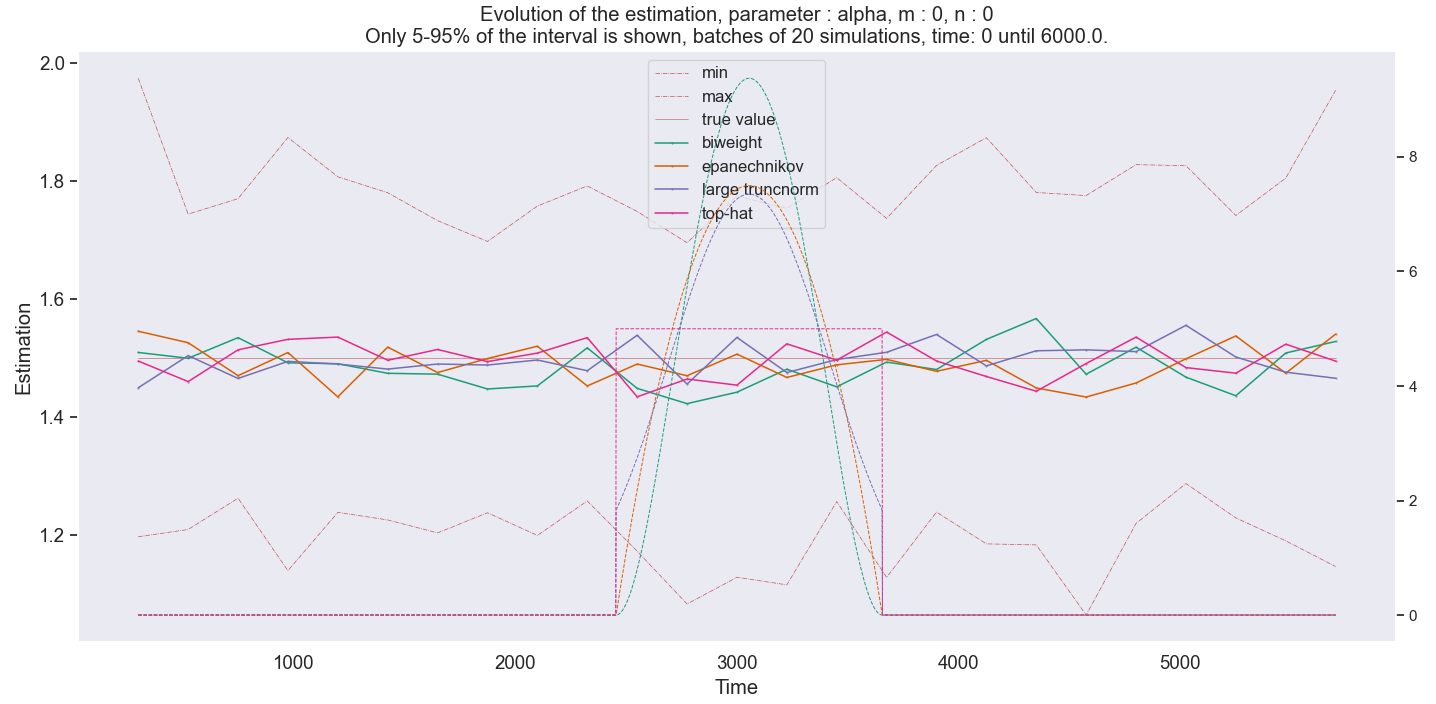
\includegraphics[width = 0.90 \textwidth]{../imag/chap3/compar_kernel/alpha.png}
\caption{Fixed kernel density estimation, showing the impact of the type of kernels. Plot of alpha. Data in \protect \path{other_estimation/4-different-kernels-over_the_time.csv}.}
\label{fig:basic_5_kernels_alpha}
\end{figure}

\begin{figure}
\centering
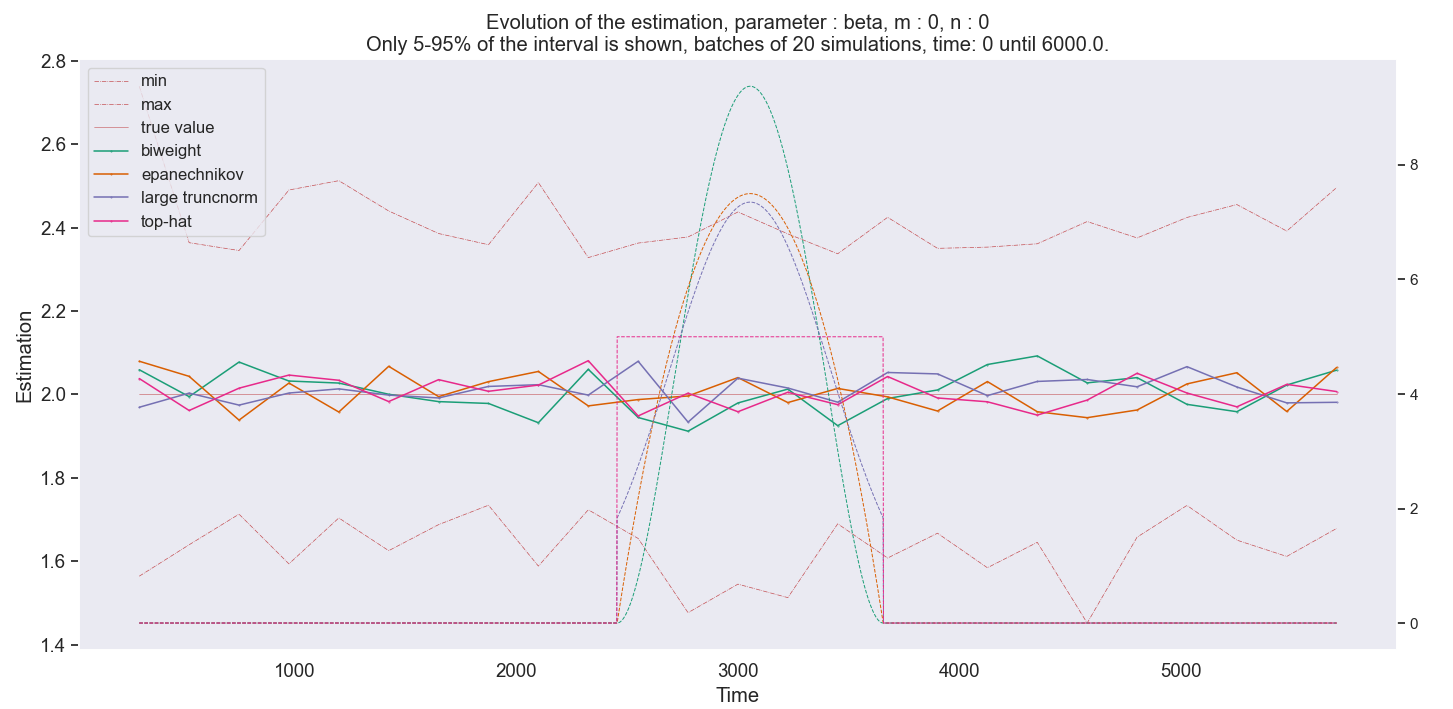
\includegraphics[width = 0.90 \textwidth]{../imag/chap3/compar_kernel/beta.png}
\caption{Fixed kernel density estimation, showing the impact of the type of kernels. Plot of beta. Data in \protect \path{other_estimation/4-different-kernels-over_the_time.csv}.}
\label{fig:basic_5_kernels_beta}
\end{figure}

\begin{figure}
\centering
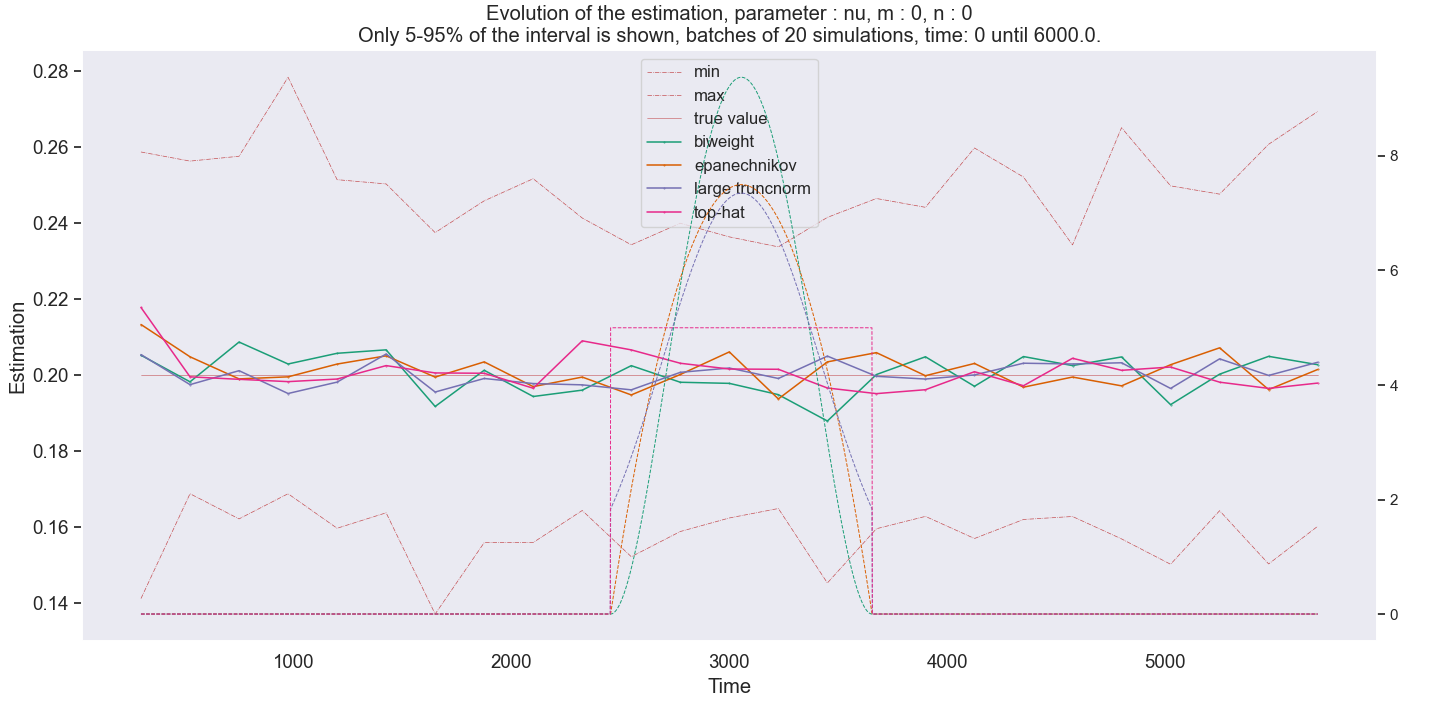
\includegraphics[width = 0.90 \textwidth]{../imag/chap3/compar_kernel/nu.png}
\caption{Fixed kernel density estimation, showing the impact of the type of kernels. Plot of nu. Data in \protect \path{other_estimation/4-different-kernels-over_the_time.csv}.}
\label{fig:basic_5_kernels_nu}
\end{figure}







\subsection{Optimal Width}
\label{subsection:optimal_width}


The optimal width derived within the theory of KDE is not relevant for our concern. The estimator $\widehat{\theta}$ is taken as a function of the kernels:

$$ \hat{f}(x) := \frac 1 {n h} \sum^n K \left ( \frac{x - X_i } {h}  \right )$$

where $n$ is the number of data you have, $h$ the window's width. However, in our case, the kernel is shaping the data given to the MLE and so the relationship between the estimate and the kernels is more ambiguous.


Since we weren't able to determine a simple relationship, we recommend choosing a meaningful width for the first optimal width. A good first blind guess can be $1/5$ of the total length of observations. The more the parameters are varying with respect to time, the smaller the width should be. That first guess about the shape of the functions driving the parameters is perhaps the most meaningful first optimal width.

\begin{remarque}
One should be careful about not having too narrow kernels. If the algorithm doesn't have enough data to observe, the MLE will give estimations with more variability and might even fail to converge.
\end{remarque}

We observe the impact of the width here in fig. \ref{fig:basic_3_kernels_alpha}, \ref{fig:basic_3_kernels_beta}, \ref{fig:basic_3_kernels_nu}. We compare the same size as the previous figures with twice and half as wide. We observe that the smallest kernels yields the more variable estimates.

\begin{figure}
\centering
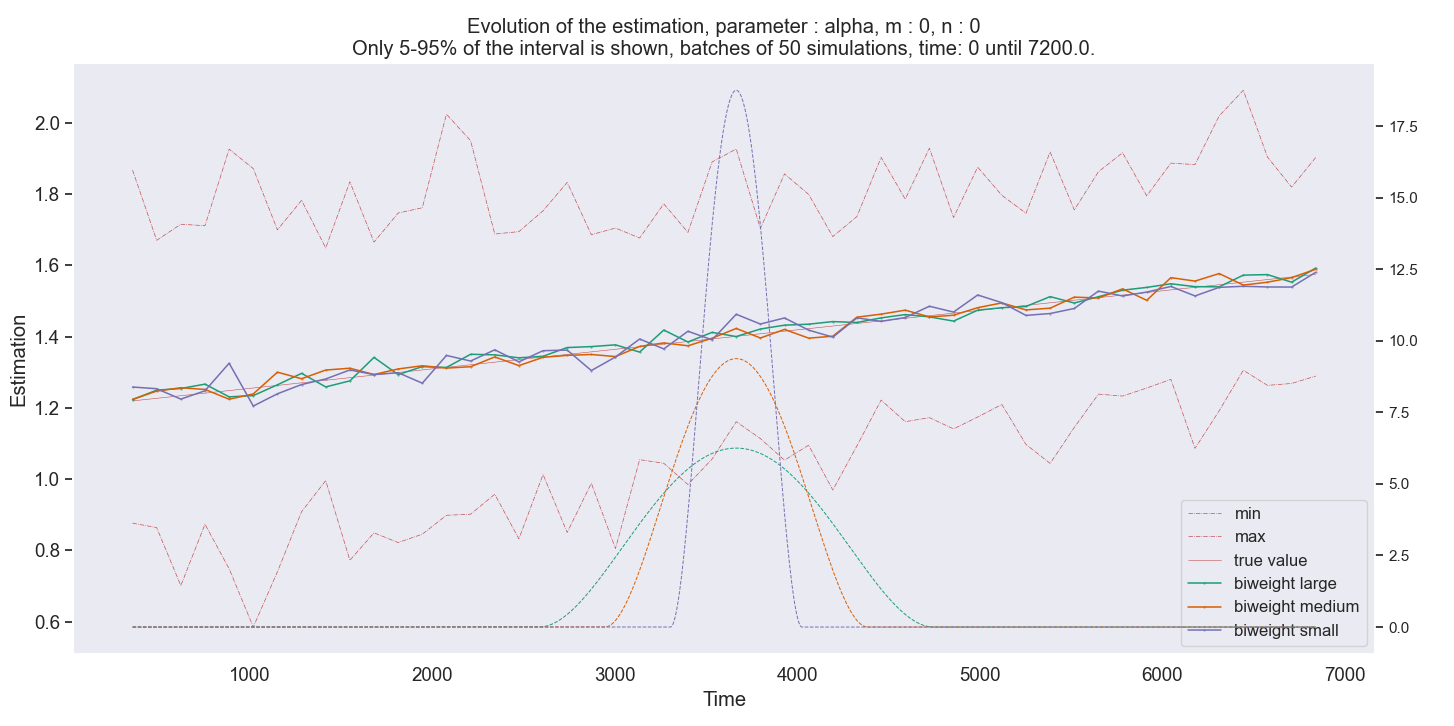
\includegraphics[width = 0.90 \textwidth]{../imag/chap3/compar_kernel/3alpha.png}
\caption{Fixed kernel density estimation, showing the impact of the width of the biweight kernel. Plot of alpha. Data in \protect \path{other_estimation/3-sizes-same-kernel-over_the_time.csv}.}
\label{fig:basic_3_kernels_alpha}
\end{figure}

\begin{figure}
\centering
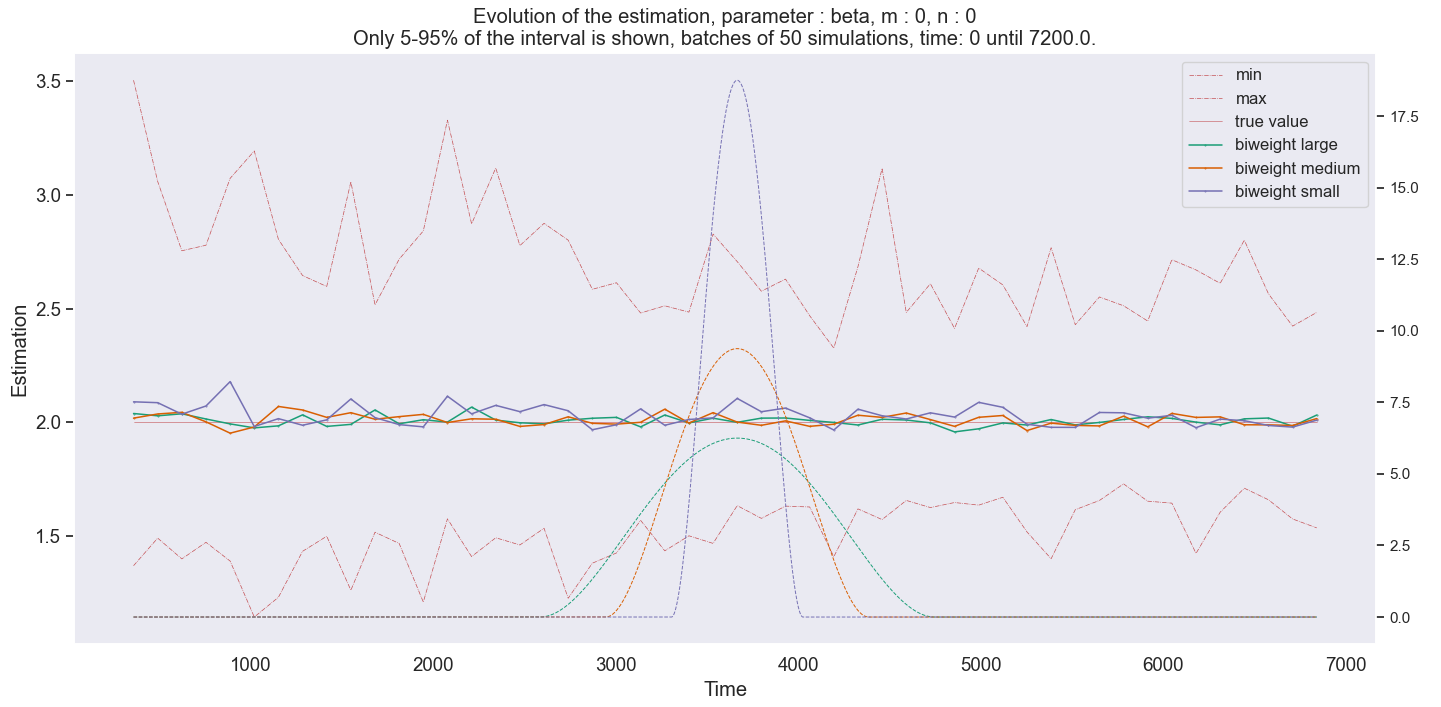
\includegraphics[width = 0.90 \textwidth]{../imag/chap3/compar_kernel/3beta.png}
\caption{Fixed kernel density estimation, showing the impact of the width of the biweight kernel. Plot of beta. Data in \protect \path{other_estimation/3-sizes-same-kernel-over_the_time.csv}.}
\label{fig:basic_3_kernels_beta}
\end{figure}

\begin{figure}
\centering
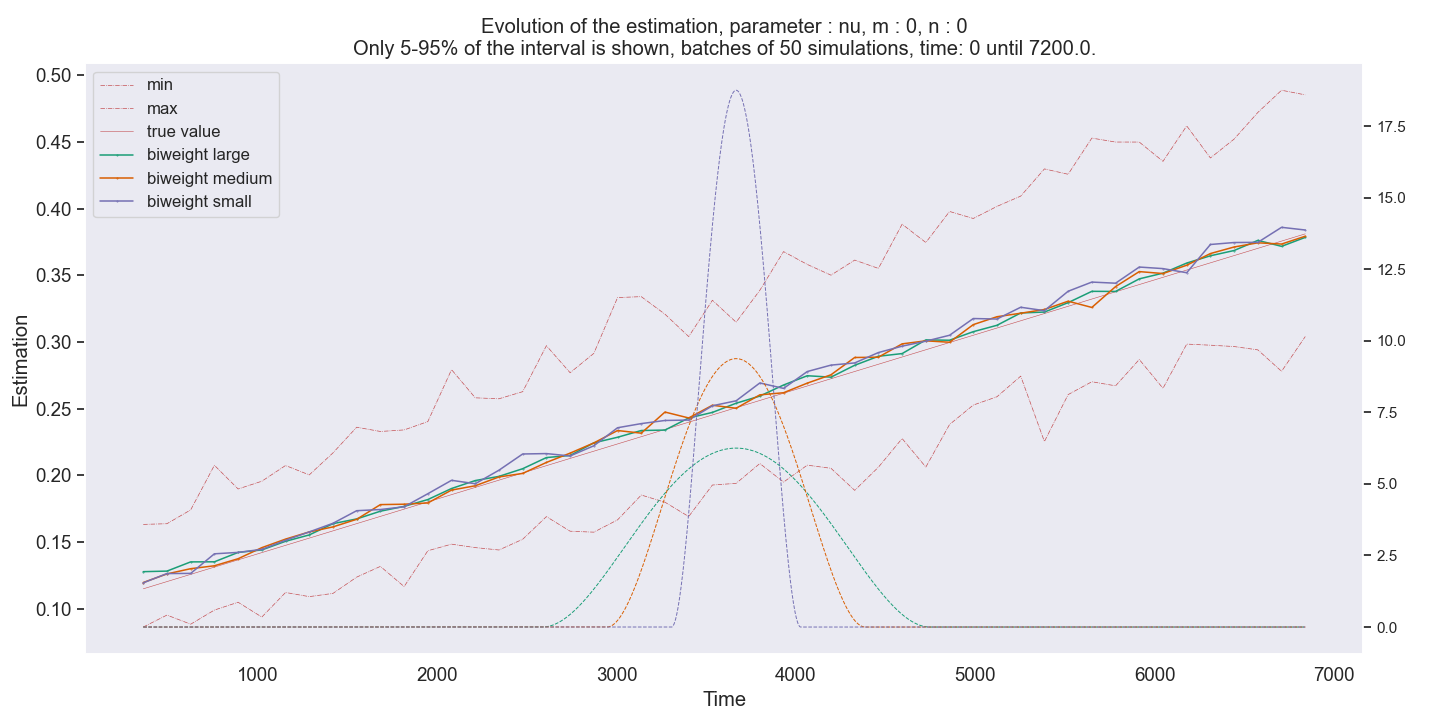
\includegraphics[width = 0.90 \textwidth]{../imag/chap3/compar_kernel/3nu.png}
\caption{Fixed kernel density estimation, showing the impact of the width of the biweight kernel. Plot of nu. Data in \protect \path{other_estimation/3-sizes-same-kernel-over_the_time.csv}.}
\label{fig:basic_3_kernels_nu}
\end{figure}




\section{Adaptive Width Window}
\subsection{Idea Behind AKDE}
Another method for KDE is called the Adaptive Kernel Density Estimation (AKDE). The author refers to \cite{Methods_ESTIM} and \cite{AKDE_ex} for more details. We synthesize the method.


Adaptive Width Window kernel estimation lies upon the idea that we are going to estimate the function through a two-step process. The first step is giving a rough estimate named the pilot estimate. Armed with the first estimate, one rescales kernels' width with respect to the geometric metric. Geometric mean has the property of being very sensible to small number. Scaling by comparing the value to the geometric mean is then a way to boost the evolution of relatively extremal values. 
Then, the second step is using the new constructed kernels in order to create a good estimate.



\subsection{Algorithm for AKDE}
\label{section:algo_awke}
The geometric mean for a sequence $\sequence{ a_i } $ is commonly defined as $$ G_{a} := \left (  \prod^n a_i \right  )^{\frac 1 n }$$ and we define the sensitivity parameter satisfying $ 0 \leq \gamma \leq 1$. It is quite common to set $\gamma = \frac 1 2$; this value can be found in the book \cite{Silverman} or in the article \cite{abramson}. Then we have:
\begin{equation}
\label{eq:local_width_factor}
\forall t_i \in \sequence{t_i}, \qquad \lambda_{t_i} :=  \left ( \frac{\widetilde{f}(t_i) }{G_{\widetilde{f_i}} } \right ) ^{ - \gamma }  
\end{equation}

and  $ G_{\widetilde{f_i}} $ is based upon the sequence $ \sequence{ \widetilde{f}(t_i) } $






\begin{algorithm}[H]
\label{algo:adaptive1}
\SetAlgoLined
1. \quad Find a pilot estimate coined $\widetilde{f}$. We use the arbitrary kernel from section \ref{section:FWW}, which for a kernel $K^*$ and a bandwidth $h^*$ is of the form $$ (t, t_i) \to \frac 1 {h^*} K^* \left ( \frac{t - t_i}{h^*} \right ) $$ 

2. \quad $\forall t_i \in \sequence{t_i}$, when we estimated the pilot estimate $\widetilde{f}$, create the local width factor $\lambda_{t_i}$ according to eq. (\ref{eq:local_width_factor}). 

3. \quad Find the final estimate $\hat{f}$ by using a different kernel for each $t_i$. $\forall t \in \sequencetime $, the new kernel shall be of the form:
$$ (t, t_i) \to \frac 1 {\lambda_{t_i} h^*} K^* \left ( \frac{t - t_i}{\lambda_{t_i} h^*} \right )$$ 
\caption{Adaptive Kernel Estimation.}
\end{algorithm}












\begin{remarque}
The interpretation of the scaling coefficient $\sequence{\lambda_{t_i}}$ can be stated like that. The bigger the coefficient, the more the bandwidth is scaled up. A coefficient smaller than one is equivalent to a pilot value bigger than the geometric mean. In other words, $\gamma$ is increasing the discrepancy of the first optimal estimate. Hence, when the estimate is relatively smaller (resp. bigger), the kernels get wider (resp. tighter). 

Essentially, such kernels are useful for KDE since places with estimated high density get narrower kernels for a more precise estimation while other intervals with low density, mainly the tails, observe wider kernels that capture the potential smooth decay of the density. 
\end{remarque}



In order to compute the geometric mean in an optimized way in python, one can use:

\begin{verbatim}
from scipy.stats.mstats import gmean
gmean( [np.array] )
\end{verbatim}

In particular, a classic problem for large arrays is overflow. A good habit is to map the array to a log-domain first, calculate the sum of these logs, then multiply by $\frac 1 n$ and finally calculate the exponential. Here I give two hand-written functions in order to compute the same result:

\begin{verbatim}
def geo_mean(iterable):
    a = np.array(iterable)
    return a.prod()**(1.0/len(a))
\end{verbatim}    
\begin{verbatim}
def geo_mean_overflow(iterable):
    a = np.log(iterable)
    return np.exp(a.sum()/len(a))
\end{verbatim}



\begin{figure}
\centering
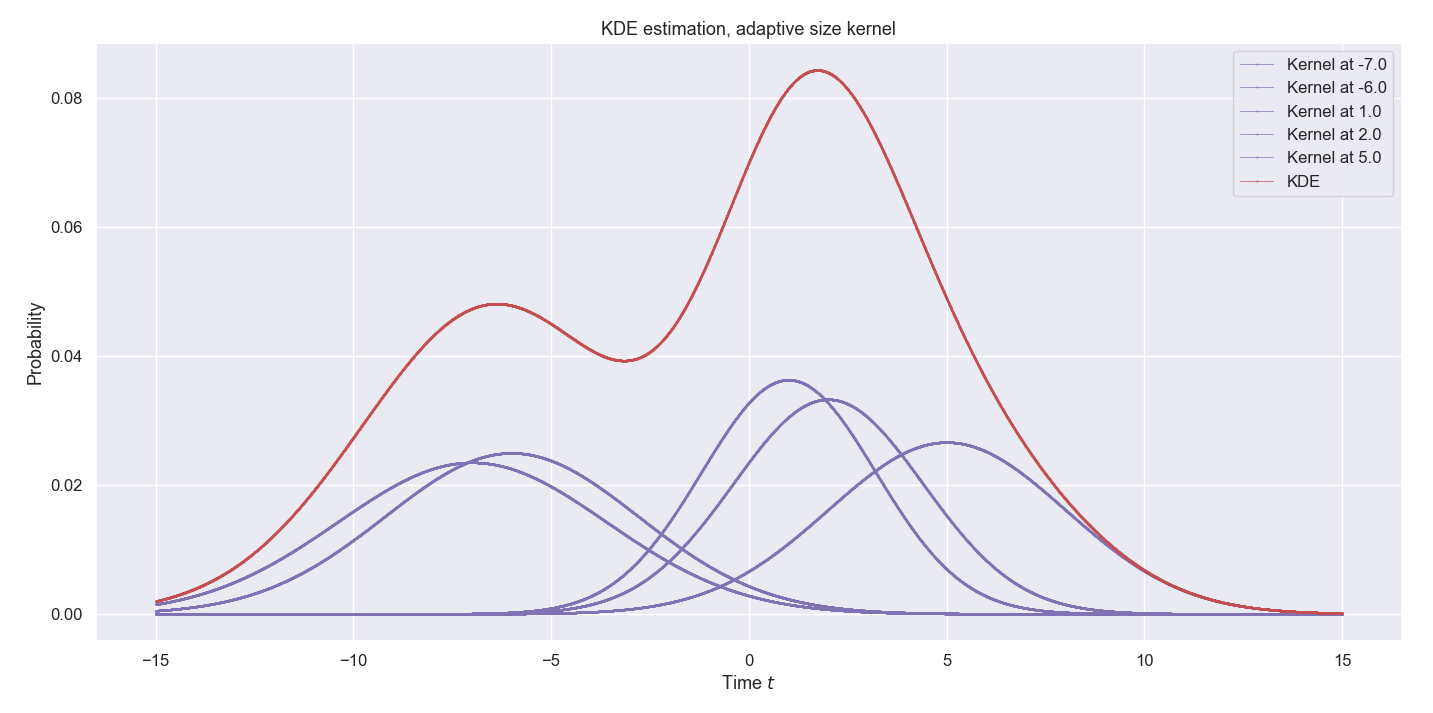
\includegraphics[width = 0.90 \textwidth]{../imag/chap3/AKDE.png}
\caption{The adaptive kernel density estimation, after the second step. Same points as on fig. \ref{fig:FKDE}), we observe how the kernels changed through the computations as well as the impact of the single kernels on the KDE.}
\end{figure}







\subsection{Equivalence Between Representation of Kernels}
\label{section:equivalence_bi_rep}

In the theory of kernels, most of plots show how one can find an estimate of a density by summing up rescaled-centred kernels, and plots like the left one from fig. \ref{fig:CKDE} are rampant. One should notice that it is also totally equivalent to represent KDE as the right picture. The rescale put aside, a kernel is a two-dimensional function: 

\begin{equation*}
(t,t_i) \to K(t - t_i) 
\end{equation*}

The left graph from fig. \ref{fig:CKDE} shows the function 
$$ \forall t \in \R, \ (t,t_{ \{1,2,3 \} }) \to K(t- t_{ \{1,2,3 \} }) $$ 
for three different $t_i$; the right one shows the function
$$ \forall t_i \in \sequence{ t_i }, \ (0,t_i ) \to K(0 - t_i) $$ 
and the stars corresponds to values we add up in order to get the estimate in $0$, when one uses $\hat{f}(t) = \sum_i K(t-t_i)$. 

This has an interesting implication. One can think about kernels as a function of one parameter and this will give a different representation of the situation depending which we chose. In the author's opinion, the second representation, from fig. \ref{fig:CKDE}, is more intuitive and efficient for our weighting problem. 

\begin{itemize}
\item Indeed, it is very \textbf{intuitive} to see the point $t$ as the point when we search for an estimate, and observe the shape of the kernel impacting the data upon it. 
\item It is also very \textbf{efficient} when one uses it with adaptive kernel estimation. The previously introduced algorithm used in KDE is based upon the first representation and thus considers the kernels as function of time. Hence, in the first representation from fig. \ref{fig:CKDE} we are scaling $\# \sequence{t_i}$ kernels, where $\#$ denotes the number of elements of the sequence. On the other hand, the other representation asks for rescaling $\#\sequencetime$ kernels. 
\end{itemize}


In the end, this double representation comes from the nature of the used kernel. We are using transition probabilities (transition kernels) which can be defined as:

\begin{definition}[Transition Kernel]
Let $(\Omega, \mathcal F), ( \mathcal X, \mathcal B (X) )$ two measurables spaces. Then $$ \kappa : \mathcal F \times \mathcal B (X) \to [0, \infty] $$ is called a kernel from $\mathcal F$ to $\mathcal B(X)$ if and only if:

\begin{itemize}
\setlength{\itemindent}{3. cm}
\item $\forall B \in \mathcal B(X), t \to \kappa(  t, B)$ is measurable
\item $\forall t \in \mathcal F, B \to \kappa(  t, B)$ is a measure.
\end{itemize}
\end{definition}

Then, one can see the previously stated $K$ or $w$ as the unidimensional case of transition kernels. Notice, we could rewrite eq. (\ref{eq:weighted_log_likelihood}) in the following way:

$$ \ln W L^m( \Theta \mid \Tau ) = - \int_0^T \lambda^{m} ( s \mid \Theta , \Tau ) \kappa(t, ds) + \int_0^T \ln \lambda^{m} ( s \mid \Theta , \Tau^m ) \kappa(t, d N_s)  $$

\begin{figure}
\centering
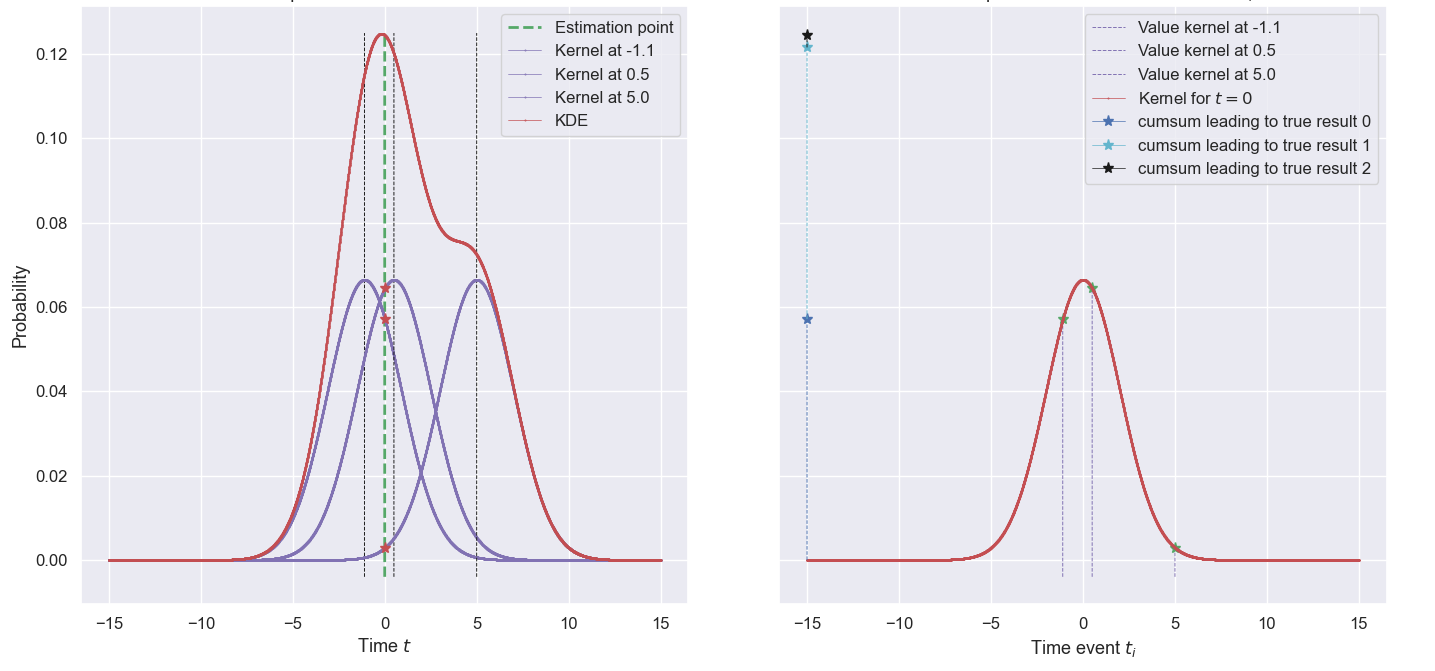
\includegraphics[width = 1.00 \textwidth]{../imag/chap3/CKDE.png}
\caption{Comparison of the two equivalent representations for symmetric kernels. The graphs share the same y-scale. On the left, one observes three kernels as function of the time and evaluated for specific $t_i$. On the right, the weight function is plotted, as a function of the events' time, for a fixed time $t$ ( $t= 0$, corresponding to the green line on the left), as well as the sum of the three points at which we evaluated the weight function. We observe that both representations lead to the same value.}
\label{fig:CKDE}
\end{figure}

\begin{figure}
\centering
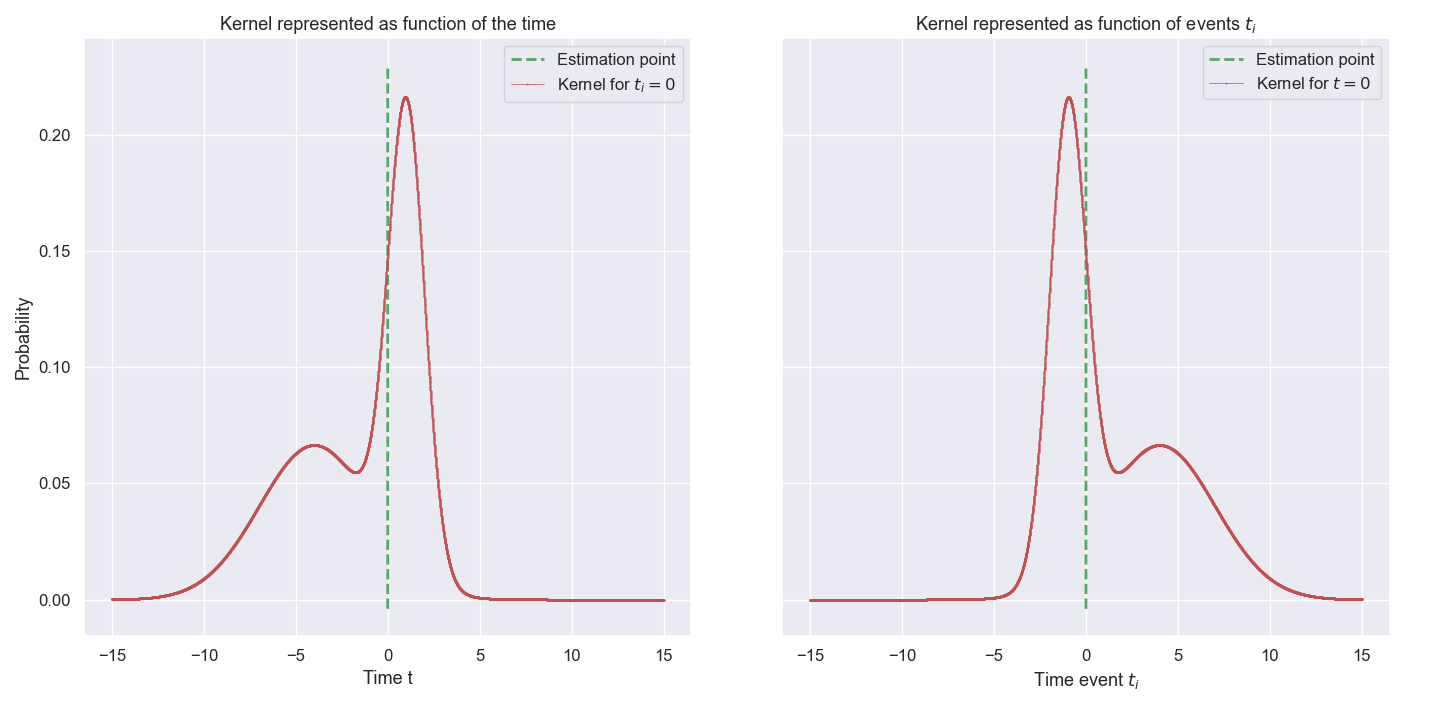
\includegraphics[width = 1.00 \textwidth]{../imag/chap3/CKDE2.png}
\caption{Kernels as function of the first or of the second argument. One is the symmetric version of the other with respect to the green dotted line.}
\label{fig:CKDE2}
\end{figure}

\willlastcheck{check that the newpage is ok.}

\newpage 
Finally, one shouldn't jump from one representation to another without some precautions. The equality $K(t - t_i) = K(t_i - t)$ holds if and only if $K$ is even. Then, though our equivalence from fig. \ref{fig:CKDE} was suggesting the usage that we plotted the same function on both plots (resp. in purple on the left and in red on the right), it is clear on fig. \ref{fig:CKDE2} that it is not the case. For that reason, the author offers to conclude the discussion we started at the end of section \ref{section:kernel_weights_first_conversation}. We wrote down the following definitions as being the main distinction between kernels and weights, which also grants some unification between the two representation:
\begin{definition}[Kernel]
$K$ is a scaled function of the time, with as parameter the jump's time $t_i$.
\end{definition}

\begin{definition}[Weight function]
$w$ is a function of the jump's time, with as parameter time $t$.
\end{definition}

\begin{theoreme}[label = thrm:equiv_w_k]{Equivalence weights and kernels}
The two definition are linked through those equalities
\begin{align*}
\forall t \in \sequencetime, \ t_i \in \sequence{t_i }, \qquad w_t(t_i) 
&= w(t_i - t) \\
&=  K(t - t_i) \cdot \norm{w}_{L^1} \\
&= K_{t_i}(t) \cdot \norm{w}_{L^1}
\end{align*}
\end{theoreme}





\section{AKDE's algorithm for WMLE}
\subsection{A New Scaling Function}



\begin{figure}
\centering
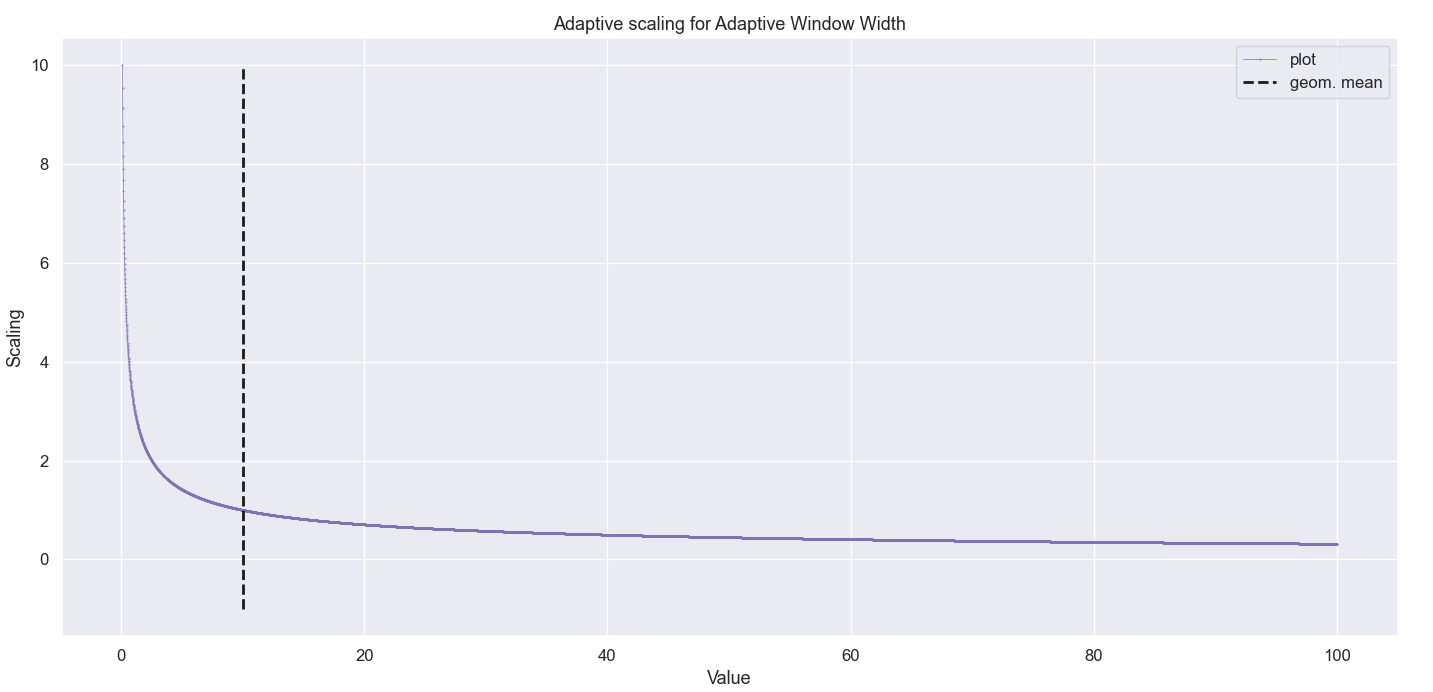
\includegraphics[width = 0.95 \textwidth]{../imag/chap3/old_funct.png}
\caption{Plot of the previously presented function $g$ in eq. (\ref{eq:local_width_factor}) as well as in equation (\ref{eq:old_g}). We plot it as a function of the first estimate's result.}
\label{fig:old_scaling}
\end{figure}


\begin{figure}
\centering
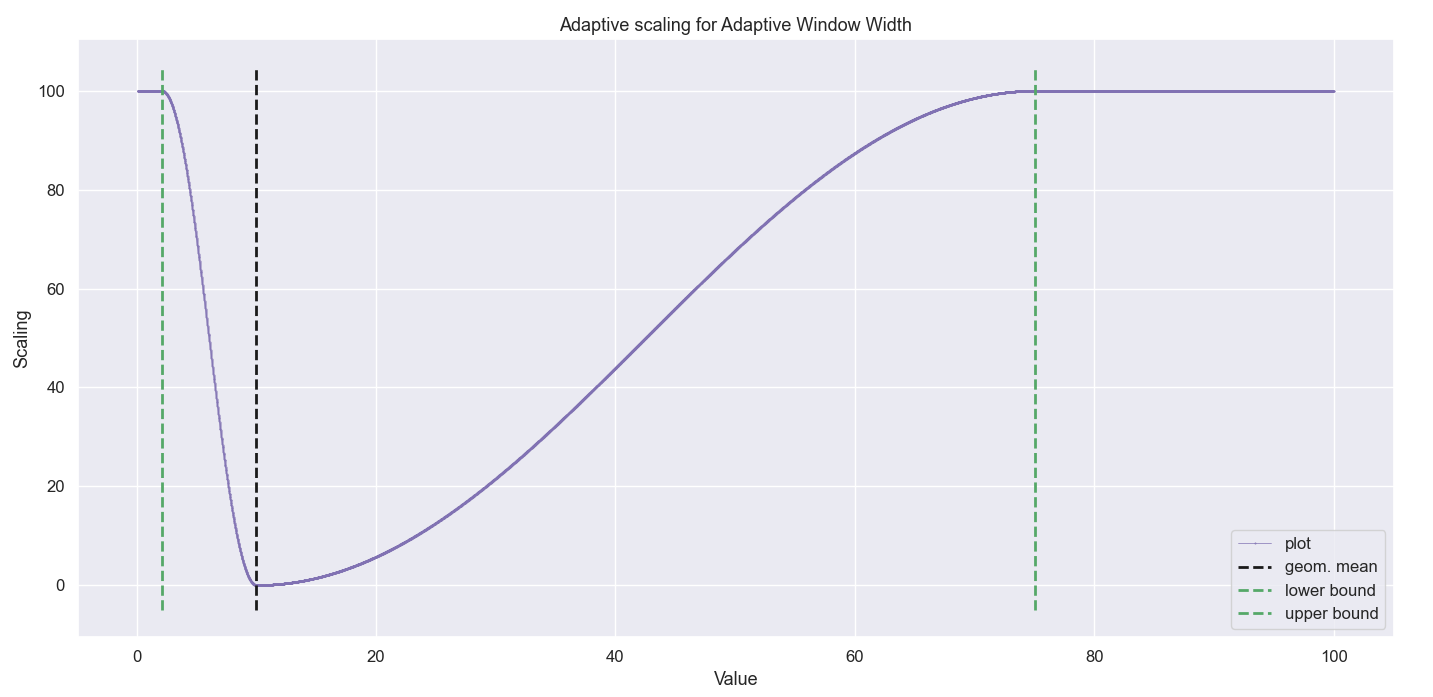
\includegraphics[width = 0.95 \textwidth]{../imag/chap3/my_new_funct.png}
\caption{Scaling output depending on how close the estimate is to the geometric mean. The lower branch ends at $2$, the mean is $10$ and the upper branch finishes at $75$. We constructed the function as a two sinusoidal branches function.}
\label{fig:new_scaling}
\end{figure}

In the previous algorithm, by observing a first estimate of the density, there was an adaptive algorithm that was able to automatically rescale the windows and give more precise results. The kernels are scaled with respect to the geometric mean. 

We observed that high probability points get narrower kernels, and low probability points get wider kernels. It makes sense in the case of AKDE. 

However, for parameter estimation in WMLE we would like to scale kernels depending on whether they are extremes, by narrowing them, and broaden kernels at points close to the average.

For that reason, we inspired ourselves from that theory and by changing the rescale function and adapting the algorithm, we came-up with a new algorithm called HATDEP\footnote{HATDEP stands for Hawkes Adaptive Time Dependent Estimation of Parameters.}. We keep the basic idea of the algorithm, being that we rescale the kernels based upon a function $g$, which takes as parameters one element of an array and the geometric mean. 

The originally used $g$ function can be written like eq. (\ref{eq:old_g}) and is plotted for $G = 10$, $\gamma = 1/2$ on fig. \ref{fig:old_scaling}. 

\begin{equation}
\label{eq:old_g}
g(x,G, \gamma) =  \left ( \frac x G \right ) ^{-\gamma}
\end{equation}

We call the function $g$ a rescale function. We want to find a better rescale function, that suits better our needs. We propose the following function:


\begin{theoreme}[label = thrm:new_g]{New $g$ rescale function}
\begin{align}
\label{eq:new_g}
g(x, G, L,R,h,l) &=   \frac {h-l} 2 \left (2 
-  \11charac_{ [- \pi, 0]} (u)  \cos(u)
-  \11charac_{ [0, \pi]} (v)  \cos(v) \right ) + l,  \\
\quad & u = \frac{x - G}{G- L} \pi, \notag  \\
\quad & v = \frac{x - G}{R- G} \pi \notag
\end{align}

For that function, $G$ shall be the junction point between the two branches. $L$ and $R$ are the end of the varying part and hence outside $[L,R]$, the value of the function $g$ is fixed. It is clear that L < G < R for the function to be well defined. We search for conditions in subsection \ref{subsection:self-defin}.
\end{theoreme}

$G$ shall correspond to the geometric mean of the pilot estimate, $L$ and $R$ are taken in the following as some quantiles of the data. $h,l$ are added as the parameter of scaling.

Recall that $p$-quantile for an ordered serie of length $n$ is defined as being equal to its $\lceil{np}\rceil$-value\footnote{$\lceil{\cdot}\rceil$ is the ceil-function.}.


What has been done here is that we created on a function that:



\begin{itemize}
\item equals to $l$ in $G$, 
\item behaves smoothly along the line, quadratically near the ends of the branches and linearly in the middle (since the function is formed of cosinus),
\item equals $h$ for extreme values,
\item is easily adaptable to the first estimation, by modifying $L$ and $R$,
\item through the substitution $u,v$, one can easily interpret R and L as the values at which the branches are reaching their final values. Choosing L and R as quantiles allows the user to choose how much data is considered as extreme. 
\end{itemize}

\begin{remarque}
We recommend taking $h$ in the interval $[1,5]$ depending on the amount of data one has. The smaller the window, the more imprecise the estimate; In fact, it makes sense that $l$ changes depending on the width of the first kernels, in order that the widest second step kernels cover the whole observation period. Hence, we use $$l = \frac{ \text{first width} }{2* \text{T max} }$$

with such value, the widest second step kernels get the width $\text{T max}$
\end{remarque}


\begin{remarque}
$L$ and $R$ and quantiles should be chosen according to a guess about the shape of the function. $4$ and $96 \%$ are good in practice, but should be increased (resp. lowered) if there are relatively many values (low values) of the type "small" for $L$ and "high" for $R$. 

The function $g$ is flat on the sides and for that reason, choosing $2$ and $98$ could also be done. 

Albeit only $4\%$ of the values being considered as extremes is not much, the number of points having the kernels narrowed is actually much bigger in practice, due to the flat behaviour of $g$ near the end of the branches. Putting $10-90$ did actually yielded half of the kernel being extremely narrowed in most cases.
\end{remarque}





One can see how the function $g$ looks like on fig. \ref{fig:new_scaling}. We offer here one implementation in python:


\begin{Verbatim}[fontsize=\footnotesize]
def mean_list(my_list):
    # the default behaviour if list is empty, it returns 0.
    return float(sum(my_list)) / max(len(my_list), 1)
    
    

def my_rescale_sin(value_at_each_time, L=0.02, R=0.98, h=2.5, l=0.2 / 2, silent=True):
    if any(value_at_each_time != 0):
        # I compute the geometric mean from our estimator.
        G = gmean(value_at_each_time)

    else:  # G == 0, it happens if no norm computed.
        # then it has to return 0.01 such that it widen all the kernels.
        return np.full(len(value_at_each_time), 0.01)

    L_quant = np.quantile(value_at_each_time, L)
    R_quant = np.quantile(value_at_each_time, R)

    if not L_quant < G < R_quant:
        raise Error_not_allowed_input("L < G < R for the well definiteness of the function.")

    if not silent:
        print("Left boundary : ", L_quant)
    if not silent:
        print("Right boundary : ", R_quant)

    xx = value_at_each_time - G

    ans = 0
    scaling1 = math.pi / (G - L_quant)
    scaling2 = math.pi / (R_quant - G)
    # I fix the part outside of my interest, to be the final value, h.
    # This part corresponds to math.pi.
    # I also need the scaling by +h/2 given by math.pi

    # xx2 and xx3 are the cosinus, but they are different cosinus.
    # So I fix them where I don't want them to move at 0 and then I can add the two functions.
    my_xx2 = np.where((xx * scaling1 > -math.pi) & (xx * scaling1 < 0),
                      xx * scaling1, math.pi)  # left
    my_xx3 = np.where((xx * scaling2 > 0) & (xx * scaling2 < math.pi),
                      xx * scaling2, math.pi)  # right
    ans += - (h - l) / 2 * np.cos(my_xx2)
    ans += - (h - l) / 2 * np.cos(my_xx3)

    ans += l  # avoid infinite width kernel, with a minimal value.
    return ans
\end{Verbatim}



\subsection{Is The Rescale Function Well-Defined ?}
\label{subsection:self-defin}

\willprecise{do a better job here}



The function $g$ should be well defined. An issue might arise if some values were negatives, but in our study, we deal with self-exciting Hawkes processes whose parameters are all positive (also, the sequence that we use for the geometric mean is the one given by the $l^2$ norm of the parameters, which is obviously positive). Another concern is, when do we have $L \leq G \leq R$? This is fundamental for the function to be well behaved. For now, the user should check it by hand. An error is thrown when it is not the case.


That question is left to the reader. As a hint, we thought about the following inequalities, which hold for any sequence of positive numbers $\sequence{a_i}$:
\willlastcheck{ Good position of the inequalities }
\begin{alignat}{2}
\text{Harmonic Mean} 
&\leq \text{Geometric Mean} 
&& \leq \text{Arithmetic Mean} \notag \\
\frac n {\sum^n \frac 1 {a_i} } 
& \leq \hspace{0.55 cm} \left ( \prod^n a_i \right ) ^{ \frac 1 n } 
&& \leq \frac 1 n \sum^n a_i \notag
\end{alignat}
where the equality holds when the sequence is constant.


















\section{From KDE to WMLE}

We mentioned throughout our study that though we summarize methods about KDE, it is actually possible to use the same methods for weighted maximum likelihood estimation. Let's go through the small necessary adjustments again.

\subsection{From Kernels to Weights}
As mentioned in section \ref{section:kernel_to_weights}, as well as through theorem \ref{thrm:equiv_w_k}, in order to go from the kernels of the theoretical part of this chapter to the space $\Omega_w$ as defined at the beginning of the chapter, one simply has to multiply by a constant, equal to the total considered time of simulation. Thus, we have the equality:

$$ T \cdot K ( \cdot ) \equiv w ( \cdot ) $$

\subsection{From One-Dimensional Kernel to Multi-Dimensional Statistics}
As mentioned in section \ref{section:multi_to_uni}, another issue lies in the fact that we can't compute the geometric mean of $\theta^*_{\cdot} \in \mathbb R^{m+2m^2}$ for the algorithm from section \ref{section:algo_awke}\footnote{By $\theta^*_{\cdot}$ we mean the function $\theta^*$, evaluated at an unknown point. The function corresponds to the estimate of the WMLE, which is a function of time because of the time dependence of the involved weights.}.
However, one can apply the geometric mean on the norms of the estimators. By default, one can use the $l^2$ norm of $\theta^*_{\cdot}$, in other words

$$\theta = (\theta_1, \theta_2, \cdots, \theta_n ) \implies 
\norm{\theta}_{l^2} = \left ( \sum^n_1 \theta_i^2 \right )^{\frac 1 2}$$ 

Please remember that in our case, $\theta$ is time dependant so taking the norm over $\theta$ recovers a function from $[0,T]$ to $\R$. Hence, if we allow $t$ to take only certain given values, $\norm{\theta_t}_{l^2}$ can be seen as a sequence.


\begin{remarque}
A particular care about the scaling of the parameters should be given. Indeed, not scaling the parameters could lead to the classic problem of data-sciences related to feature standardization. The features with high magnitudes will weight a lot more in the distance calculations than features with low magnitudes, in particular with the euclidean distance.
\end{remarque}

\subsection{Scaling}
\label{subsection:scaling}

As mentioned in the previous subsection, we might have to apply some scaling to the estimates. Indeed, the results are sensitive to the relative scaling. We chose a classical positive mean-scaling:

\begin{equation}
\forall i \in  \llbracket 1, M \rrbracket, \qquad  \widetilde{\theta_i } = \frac{\theta_i - \mean \theta }{\max(\theta) - \min(\theta) } + 1 
\label{rescale-function}
\end{equation}

It makes sense as we care about how the values are extremes in comparison to each others. The scaling is also linear and thus does not change essentially the distribution\footnote{Unlike normalization.}. 

The classical mean-scaling does not involve the additional $+1$, and its values lie in $[-1,1]$. The shift ensures a positive value, which is very important in order to keep the order of norms, without which the rescale function $g$ can't work properly. By adding 1 to the scaling, we move the domain to only positive values, on which the norm is monotone. On the other hand, the norm is not monotonous on $[-1,1]$. 


A problem appears with non-moving parameters. Worst case scenario is when there is no change for a parameter. Then, the time series of means is showing no autocorrelation and the plot is essentially noise. Furthermore, it is quite common to observe some strong correlation in between the parameters (alpha goes up, beta goes up as well) exaggerating the change in the kernels' width. A solution we implemented is to not consider the evolution of parameters with no significant change. Our criteria is a minimal percent change with respect to the original (at time 0) value of the parameter. The default minimum is $10\%$ though it can be changed.


We offer here an implementation of what we just have said. 

\begin{Verbatim}[fontsize=\footnotesize]
def rescale_min_max(vect):
    the_max = max(vect)
    the_min = min(vect)
    the_mean = classical_functions.mean_list(vect)
    ans = [(vect[i] - the_mean) / (the_max - the_min) + 1 for i in range(len(vect))]
    return ans


def check_evoluating(vector, tol):
    ''' if all values of the vector are inside the tube mean +/- 
    '''
    the_mean = classical_functions.mean_list(vector)
    if all(element < the_mean * (1 + tol) for element in vector) and all(
            element > the_mean * (1 - tol) for element in vector):
        return False
    return True


def rescaling_kernel_processing(times, first_estimate, considered_param, tol=0, silent=True):
    # on the first entry, I get the time, on the second entry I get nu alpha or beta, 
    #then it s where in the matrix.
    # considered_param should be which parameters are important to consider.

    # ans is my vector of normes. Each value is for one time.
    ans = np.zeros(len(times))

    # times and first_estimate same length.
    # I need to pick the good parameters and rescale them accordingly.

    # the dimension of the data.
    M = len(first_estimate[0][0])
    total_M = 2 * M * M + M
    include_estimation = [False] * total_M
    # I am creating a vector with 2M*M + M entries,
    #each one is going to be scaled, and this is the parameters I am using afterwards.
    vect_of_estimators = [[] for _ in range(total_M)]
    for k in range(len(times)):
        for i in range(M):
            vect_of_estimators[i].append(first_estimate[k][0][i])
            for j in range(M):
                vect_of_estimators[M + i + j].append(first_estimate[k][1][i][j])
                vect_of_estimators[M + M * M + i + j].append(first_estimate[k][2][i][j])

    for i in range(total_M):
        # check the parameters I need to check.
        if i < M and 'nu' in considered_param:
            include_estimation[i] = True
        elif i < M + M * M and 'alpha' in considered_param:
            include_estimation[i] = True
        elif 'beta' in considered_param:
            include_estimation[i] = True

        if include_estimation[i]:
            if not check_evoluating(vect_of_estimators[i], tol):  # we don't keep the True
                include_estimation[i] = False
    if not silent:
        print("which dim to include for norm : ", include_estimation)

    rescale_vector = []
    for i in range(total_M):
        if include_estimation[i]:
            rescale_vector.append(rescale_min_max(vect_of_estimators[i]))

    for j in range(len(times)):
        ans[j] = np.linalg.norm(
        [rescale_vector[i][j] for i in range(len(rescale_vector))], 2)
    # I compute the geometric mean from our estimator.
    G = gmean(ans)
    if not silent:
        print("vect  :", vect_of_estimators)
        # print("interm :", rescale_vector)
        print("the norms ", ans)
        # print('mean : ', G)
    scaling_factors = my_rescale_sin(ans, G=G, silent=silent)
    return scaling_factors
\end{Verbatim}

\subsection{Number of Kernels to Rescale}
As exposed in section \ref{section:equivalence_bi_rep}, both representation of the kernels are equivalent. The first one (kernels as functions of the events) is rampant throughout KDE theory, though we believe the second one is more intuitive in our case scenario.

We shall take advantage of the double representation in order to reduce computational cost. When we want to continuously evaluate a function based on discrete data, it makes sense to compute a scale variable for each element of $\sequence{t_i}$. However, in our case scenario, we want to weight our MLE at specific discrete times $\sequencetime$, using a big set of data $\sequence{t_i}$ (relatively so big that it is considered continuous). It thus makes sense to, instead of rescaling the kernels with respect to the events $\sequence{t_i}$, we shall rescale the weights with respect to the times $\sequencetime$. It drastically reduces computational costs as well as simplifies how one can implement that algorithm.




\subsection{Implementation Difficulties in Python}
There is a problem related to numerical computations. Since the interval of observed data is not infinite, there might be points where we are processing estimation, at which the support of the kernel is not strictly included inside the simulation interval. One solution would be to estimate at points for which kernels are fully included inside the interval. However, it means there are points for which we can't estimate the parameters, and it then means we lose a lot of data. On the other hand, we saw that there is a quadratic tendency in the complexity of the estimation algorithm, so we really need to use as much data as possible instead of wasting it. A solution is scaling up the kernels in order to keep the integral of it equal to $T$, as mentioned in the constraint. Then, the shape is only partially the one set, but the "energy" is conserved and the estimate is correct. One can see the impact of such scaling on fig. \ref{fig:scaling_kernels}. In order to scale up, the author did compute the numerical integral of the kernel and scale accordingly.

Also, we also mentioned the burn-in period as being compulsory in order to reach some kind of stationary behaviour for the process. It can be difficult to incorporate this period of time while skipping it for the estimation and adapt the kernels; one should be extremely careful with it.



\begin{figure}
\centering
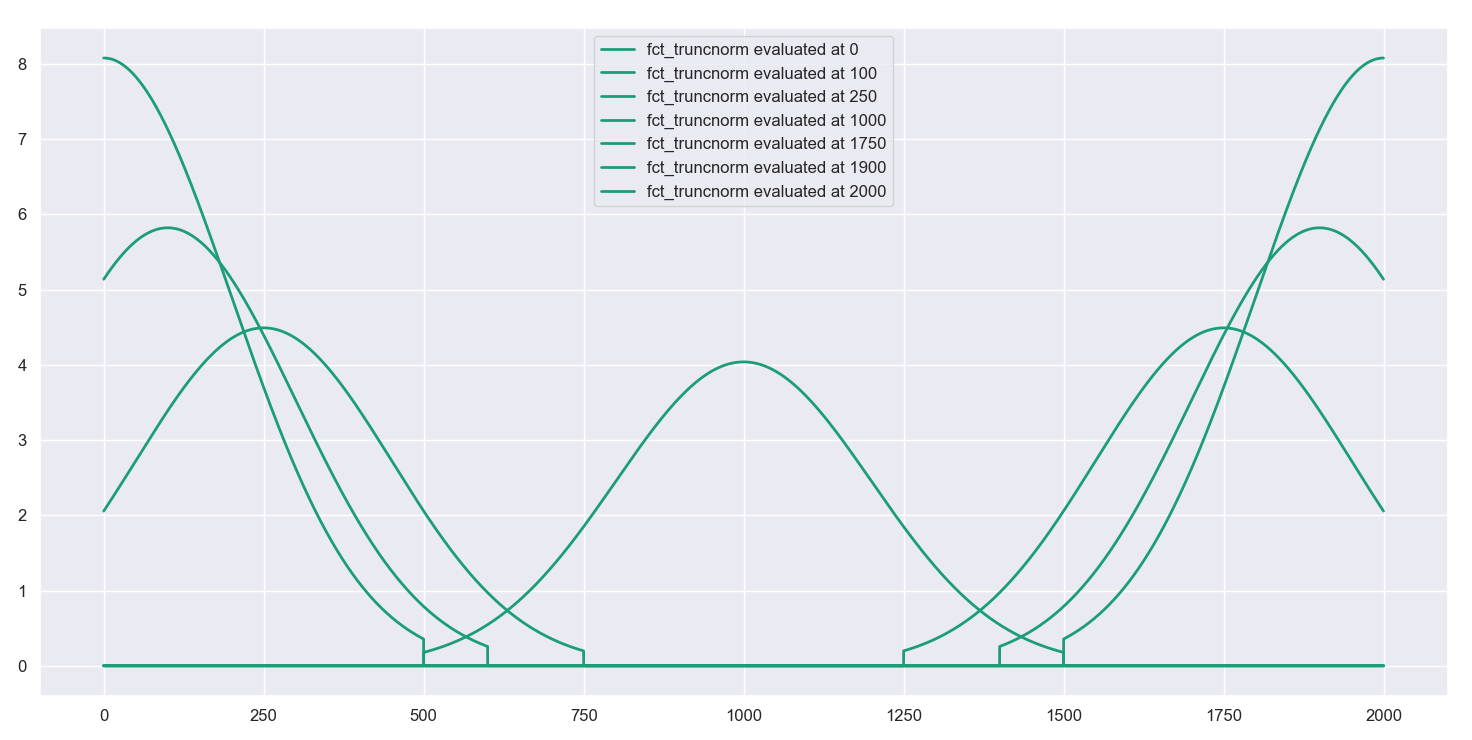
\includegraphics[width = 0.90 \textwidth]{../imag/chap2/impact_edge_kernel.png}
\caption{Shape of the kernel, depending on where it is located on the interval $[0,T]$; here $T = 2000$.}
\label{fig:scaling_kernels}
\end{figure}



\section{Sum-Up Algorithms}
\subsection{Algorithm for Adaptive WMLE: the HATDEP}
Following the algorithm \ref{algo:adaptive1}, we write our final version of the adaptive weighting algorithm. The major changes that we apply are:

\begin{itemize}
\item rescale the parameters if necessary, according to the equation (\ref{rescale-function}), for each dimension, excluding the dimensions that are non evolving,
\item rescale the weights $t$ instead of the kernels $t_i$, for computational reasons,
\item usage of the norm upon the estimate $\theta^*$\footnote{after rescaling the different coefficients as suggested.},
\item change the rescale function $g$ defined in eq. (\ref{eq:new_g}). The function $g$ is seen as a two-dimensional function; the rest of the parameters are fixed.
\end{itemize}


We then get the new scaling parameters:


\begin{equation}
\forall t \in \sequencetime, \qquad \lambda_{t} :=  
g \left (\norm{\widetilde{\theta_{t}}}_{l^2}, 
G_{\norm{\widetilde{\theta_{\cdot}}}_{l^2}} \right)   
\end{equation}

and  $ G_{\norm{\widetilde{\theta_{\cdot}}}_{l^2}} $ is based upon the sequence $\{ \norm{\widetilde{\theta_{\cdot}}}_{l^2} \} $


The algorithm becomes:


\begin{algorithm}[H]
\label{algo:adaptive2}
\SetAlgoLined
1. \quad Find a pilot estimate coined $\widetilde{\theta_t}$. We use the optimal weight from section \ref{section:FWW}, which for a weight $w^*$ and a bandwidth $h^*$ is of the form  $$ (t, t_i) \to \frac 1 {h^*} w^* \left ( \frac{t_i - t }{h^*} \right ) $$ 

2. \quad $\forall t \in \sequencetime$, when we estimated the pilot estimate $\widetilde{\theta_t}$, create the local width factor $\lambda_t$ according to eq. (\ref{eq:local_width_factor}). 

3. \quad Find the final estimate $\hat{\theta_t}$ by using a different weight for each different time $t$. 

$\forall t \in [0,T]$, the new weight shall be of the form:
$$ (t, t_i) \to \frac 1 {\lambda_{t} h^*} w^* \left ( \frac{t - t_i}{\lambda_{t} h^*} \right )$$ 
\caption{Hawkes Adaptive Time Dependant Estimation of Parameters (HATDEP).}
\end{algorithm}


\section{Other Fancy Methods}

\subsection{Adaptive window method}
Another idea, no time for that but, would be that instead of using a global scaling function, one could locally compute a coefficient for scaling. There would be a window centred around the kernel we rescale, and depending on the change in value with the estimates around, the scale would change. Then, instead of looking at the relative global value of one estimate, one rescales according to the relative variation of the estimate.

\subsection{Radial Basis Function}

I won't have time for that. There was the topic of radial basis function as well as the truncated kernels I saw in Wand. 


\willmuchlater{Need to read about method. \newline and write about it. \newline. Perhaps I won't have the time.}

\willmuchlater{ I also want to look at the truncated kernels.}






